\documentclass[14pt]{article}

\usepackage[UTF8]{ctex}
\usepackage[a4paper]{geometry}
\usepackage{amsmath}
\usepackage{fancyhdr}
\usepackage{amsthm}
\usepackage{amssymb}
\usepackage{xcolor}
\usepackage{tikzsymbols}
\usepackage{gensymb}
\usepackage{ctex} % 支持中文的LaTeX宏包
\usepackage{amsmath,amsfonts,graphicx,subfigure,amssymb,bm,amsthm,mathrsfs,mathtools,breqn} % 数学公式和符号的宏包集合
\usepackage{algorithm,algorithmicx} % 算法和伪代码
\usepackage[noend]{algpseudocode} % 算法和伪代码
\usepackage{fancyhdr} % 自定义页眉页脚
\usepackage[framemethod=TikZ]{mdframed} % 创建带边框的框架
\usepackage{fontspec} % 字体设置
\usepackage{adjustbox} % 调整盒子大小
\usepackage{fontsize} % 设置字体大小
\usepackage{tikz,xcolor} % 绘制图形和使用颜色
\usepackage{multicol} % 多栏排版
\usepackage{multirow} % 表格中合并单元格
\usepackage{pdfpages} % 插入PDF文件
\usepackage{listings} % 在文档中插入源代码
\usepackage{wrapfig} % 文字绕排图片
\usepackage{bigstrut,multirow,rotating} % 支持在表格中使用特殊命令
\usepackage{booktabs} % 创建美观的表格
\usepackage{circuitikz} % 绘制电路图
\usepackage{zhnumber} % 中文序号(用于标题)
\usepackage{tabularx} % 表格折行
\usepackage{titlesec}
\definecolor{CPPLight}  {HTML} {686868}
\definecolor{CPPSteel}  {HTML} {888888}
\definecolor{CPPDark}   {HTML} {262626}
\definecolor{CPPBlue}   {HTML} {4172A3}
\definecolor{CPPGreen}  {HTML} {487818}
\definecolor{CPPBrown}  {HTML} {A07040}
\definecolor{CPPRed}    {HTML} {AD4D3A}
\definecolor{CPPViolet} {HTML} {7040A0}
\definecolor{CPPGray}  {HTML} {B8B8B8}
\lstset{
    columns=fixed,       
    numbers=left,                                        % 在左侧显示行号
    frame=none,                                          % 不显示背景边框
    backgroundcolor=\color[RGB]{245,245,244},            % 设定背景颜色
    keywordstyle=\color[RGB]{40,40,255},                 % 设定关键字颜色
    numberstyle=\footnotesize\color{darkgray},           % 设定行号格式
    commentstyle=\it\color[RGB]{0,96,96},                % 设置代码注释的格式
    stringstyle=\rmfamily\slshape\color[RGB]{128,0,0},   % 设置字符串格式
    showstringspaces=false,                              % 不显示字符串中的空格
    language={[x86masm]Assembler},                       % 改为x86-32汇编高亮
    morekeywords={mull, divl, addb leal,xorl,pushl,popl,testl,testb,movl,movb,incl,decl,cmpb,cmpl,mov,add,sub,jmp,cmp,je,jne,push,pop,inc,dec,call,ret,lea,nop,or,and,xor,int,syscall,sysreturn},
    emph={eax,ebx,ecx,edx,esi,edi,esp,ebp,eip},
    emphstyle=\color{CPPViolet},
}

\definecolor{dkgreen}{rgb}{0,0.6,0}
\definecolor{gray}{rgb}{0.5,0.5,0.5}
\definecolor{mauve}{rgb}{0.58,0,0.82}
\lstset{
  frame=tb,
  aboveskip=3mm,
  belowskip=3mm,
  showstringspaces=false,
  columns=flexible,
  framerule=1pt,
  rulecolor=\color{gray!35},
  backgroundcolor=\color{gray!5},
  basicstyle={\small\ttfamily},
  numbers=none,
  numberstyle=\tiny\color{gray},
  keywordstyle=\color{blue},
  commentstyle=\color{dkgreen},
  stringstyle=\color{mauve},
  breaklines=true,
  breakatwhitespace=true,
  tabsize=3,
}
\setlength{\headheight}{14.49998pt}

\newtheorem{question}{\hskip 1.7mm \bf}
\renewenvironment{proof}{{\noindent\hskip 2.4em \bf ֤证明 \quad}}{\hfill$\qed$\par}
\newenvironment{solution}{{\noindent\hskip 2.4em \bf 解 \quad}}

\titleformat{\section}{\fontsize{20pt}{22pt}\selectfont\bfseries}{\thesection}{1em}{}
\titleformat{\subsection}{\fontsize{18pt}{20pt}\bfseries}{\thesubsection}{1em}{}
\titleformat{\subsubsection}{\fontsize{16pt}{18pt}\bfseries}{\thesubsubsection}{1em}{}

\geometry{left=2.0cm,right=2.0cm,top=2.5cm,bottom=2.5cm}
\begin{document}
\fontsize{13pt}{18pt}\selectfont


\pagestyle{fancy}
\lhead{中国科学院大学}
\chead{\bf{计算机组成原理}}
\rhead{\emph{2023K8009929044 薛翼舟}}


\begin{center}
\huge{\bf{现代计算机系统中典型的总线标准}}
\end{center}

本片报告将分别介绍几种现代计算机系统中典型的总线标准

\section{PCI-express总线}
\subsection{背景}
PCI express总线(下简写为PCIe)是Intel公司在2001提出的一种新的总线标准, 是基于之前传统PCI总线的高级拓展, 可以提供更高的数据传输带宽, 更大的最大系统总线吞吐量
以及更低的延迟, 更低的I/O引脚数量和更小的物理尺寸.

\subsection{基本特征}
PCIe和传统的PCI总线结构的最主要的区别是总线的拓扑结构, 传统的PCI总线是采用的并行总线架构, 而PCIe采用的策略是基于点到点拓扑, 单独地串行链路将
每一个设备直接连接到主机,极大程度上避免了总线争用的问题, 可以实现任何端点之间的全双工通信.\par
此外, 每个设备和主机相互连接的通道都包含一堆差分信号线, 支持全双工通信\par
PCIe的协议分为三层, 分别是物理层(Physical Layer)、数据链路层(Data Link Layer)和事务层(Transaction Layer), 其中
\begin{enumerate}
  \item 物理层负责比特级数据的传输, 
  \item 数据链路层负责数据的可靠传输和流量控制在数据链路层中添加了序列号,CRC校验等确认机制, 另外通过包重发机制来保证了数据不会丢失或者重复, 
  \item 事务层负责处理设备之间的通信请求和响应.
\end{enumerate}
在PCIe结构中使用数据包在设备之间传递信息,数据包在事务层和数据链路层中形成,以将信息从发送设备传送到接收设备。
\newpage
\subsection{基本结构和实现原理}
  PCIe的总线拓扑结构基本上就是一个树形的结构, 如图所示
\begin{figure}[H]
    \centering
    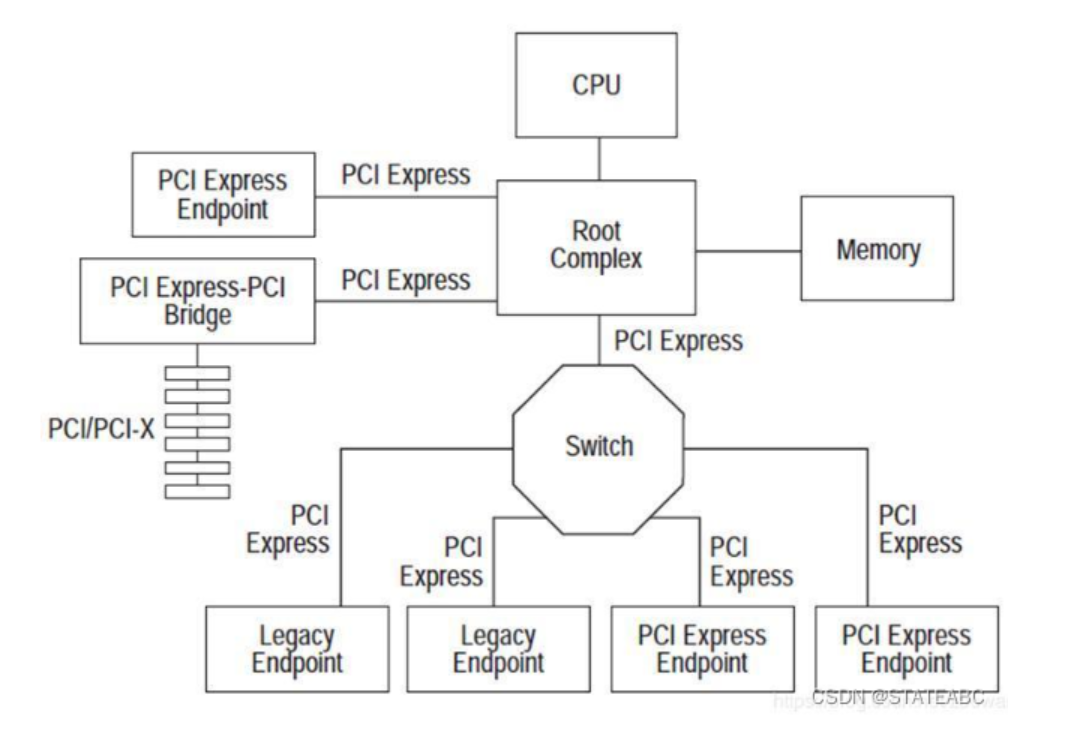
\includegraphics[width=0.8\textwidth]{pcle_1.jpg}
    \caption{PCIe总线拓扑结构}
\end{figure}
\subsubsection{Root Complex}
我们可以看到, PCIe总线的根节点是Root Complex, 它是连接CPU和PCIe设备的桥梁, 负责管理PCIe设备的访问和通信,主要功能是完成存储器域到PCIe总线域的地址转换,RC把来自CPU的request转化成PCIe的4种不同的请求
(configuration, Memory,I/O,Message)并发送给接在它下面的设备。\par
\subsubsection{Switch}
正如我们之前所说,PCIe总线协议的设备和总线之间的连接是点对点的, 这也就意味着一条PCIe链路的两端只能链接两个设备, 所以如果我们需要在
一条链路上搭载更多的设备, 就需要switch转换器进行选择\par
\subsubsection{Endpoint}
Endpoint是PCIe总线的终端设备, 它是实际的PCIe外设,它们作为数据传输的发起方或接收方\par
总的来说, 就是说RC实际上是CPU和PCIe各个设备之间的桥梁, 相当于RC将CPU发送的请求(设备向CPU发送请求同理)经过编辑, 然后经过switch转换来选取
具体的设备, 然后利用数据包进行数据和信息的传递

\subsection{典型部件}
PCIe总线标准主要用于连接各种高速设备, 如显卡、存储设备、网络接口卡等

\bigskip
\bigskip
\bigskip
\bigskip
\bigskip

\section{DDR4}
由于DDR4是DDR3的升级版, 所以我们在此支介绍DDR4和DDR4相比DDR3的进化
\subsection{背景}
DDR代表的是double data rate 也即双倍速据速率, 是最常见的主存RAM接口总线标准, 用于CPU和内存之间的数据交互\par
DDR3在2007年推出, 而DDR4在2014年推出, DDR4的主要目标是提高内存带宽和降低功耗, 以满足现代计算机系统对性能和能效的需求.
\subsection{基本特征}
DDR这种内存总线计数的最主要的特征就是双倍的数据传输速率, 在传统的数据交换中, 只有在时钟信号的上升沿或者下降沿才发生数据传输, 而DDR
技术采用的是在时钟上升沿和下降沿都传输数据, 进而就实现了双倍的传输\par
DDR4相比DDR3的提升主要是DDR4在物理接口、电压、信号完整性、频率等方面相比DDR3有明显提升, 另外DDR4引入了一个新的部件就是Bank Group,
允许每个Bank Group内的Bank可以独立访问, 进而提高了内存的并行性和性能\par
\subsection{基本结构和实现原理}
DDR采用并行数据总线,每根数据线同时传输一位数据,数据总线宽度典型为64bit(单通道),服务器平台可多通道并行\par
另外DDR结构采用了予取机制, 也即一次访问从内存阵列中读取多位的数据, 后来在按需要时分配到数据线上, DDR4的结构如下图所示
\begin{figure}[H]
    \centering
    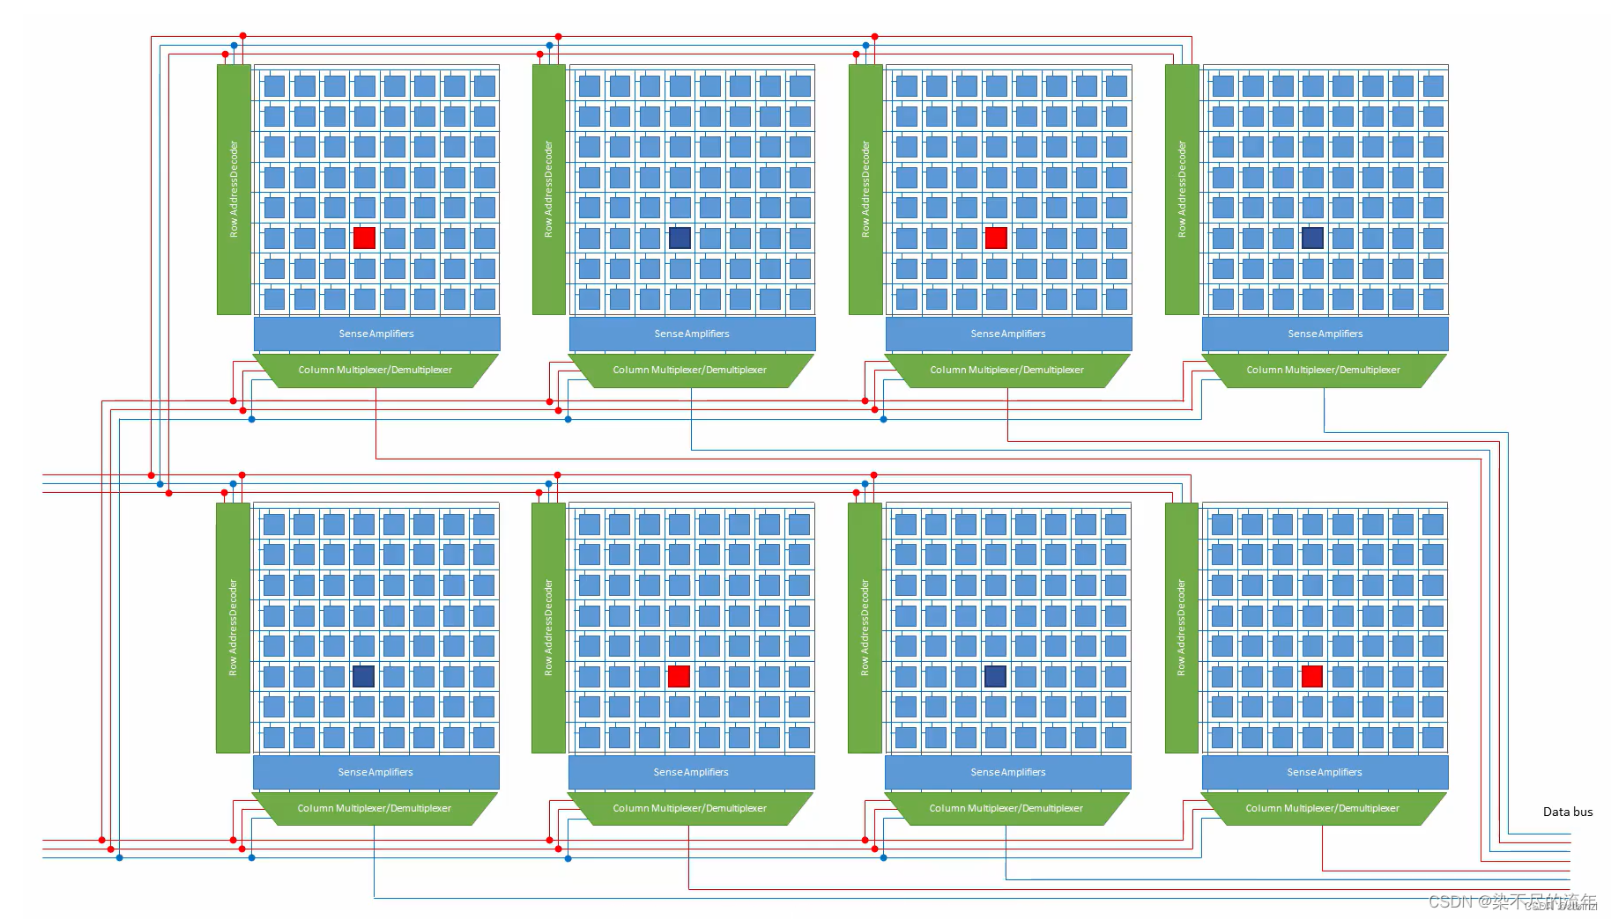
\includegraphics[width=1\textwidth]{drr4.jpg}
    \caption{ddr4的8-cell并联结构}
\end{figure}
为了进一步加速数据读写效率,DDR4将16个Cell阵列进行并联,让其共用行/列地址线,通过各自独立的16根数据线,一次可以同时读写16bit数据,
DDR4将使用此种方式并联起来的16个Cell阵列称为一个Bank。Bank内16bit数据同时读写的机制也称为数据预取,即DDR4单个Bank具备16bit数据预取能力,
大大提高了数据读写效率。\par
在此之上, 也如之前所提到的, 4个Bank组成一个Bank Group, 每个Bank Group可独立工作, 进一步地提升了内存的并行性和性能, 使得DDR4在多任务处理和高负载应用中表现更好.\par
\subsection{典型部件}
DDR4主要用于现代计算机系统的主存储器, 包括台式机、笔记本电脑、服务器等, 其主要部件包括内存条和内存控制器

\bigskip
\bigskip
\bigskip
\bigskip
\bigskip


\section{AXI总线}
\subsection{背景}
AXI总线, 也即Advanced eXtensible Interface,高级可扩展接口是ARM公司提出的AMBA(Advanced Microcontroller Bus Architecture)总线协议家族中的一种,是目前主流ARM 
SoC(System on Chip,片上系统)内部常用的高性能总线标准。是一种片内总线, 用于连接芯片内部各个部件
\subsection{基本特征}
AXI总线的一大特征是AXI的地址,控制和数据的相位是分离的, AXI支持不对齐的数据传输; 另外, AXI总线支持突发传输, 可以一次性高效地传输
大块数据, 极大程度上减少了握手的时序开销; 最后AXI总线支持乱序和多主控

\subsection{基本结构和实现原理}
AXI总线是基于主从架构的并行通信协议, 就是主设备在通道上向从设备slave发送各种信息和请求 , 然后slave根据主设备的请求进行响应, 其主从结构示意图如下所示

\begin{figure}[H]
    \centering
    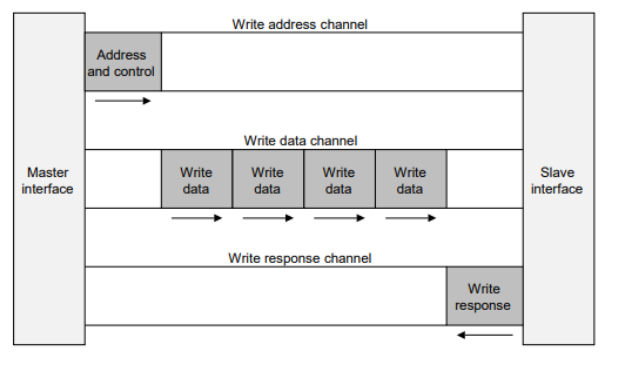
\includegraphics[width=0.8\textwidth]{AXI.jpg}
    \caption{AXI总线主从结构示意图}
\end{figure}
\newpage
具体地, AXI总线协议包括如下五个通道
\begin{enumerate}
    \item 写地址通道(Write Address Channel)\\
传送写操作的目标地址和控制信号。
\item 写数据通道(Write Data Channel)\\
传送实际要写入的数据。
\item 写响应通道(Write Response Channel)\\
返回写操作的执行结果和状态。
\item 读地址通道(Read Address Channel)\\
传送读操作的目标地址和控制信号。
\item 读数据通道(Read Data Channel)\\
返回读取到的数据和状态信息。
\end{enumerate}

AXI总线的主要工作传输流程(以读过程为例)如下
\begin{enumerate}
    \item 主设备通过读地址通道发送写请求和各个控制信号
    \item 从设备在接收到地址后, 在读数据通道上返回读到的数据
\end{enumerate}

\subsection{典型部件}
AXI总线主要用于片上系统(SoC)中的各种组件之间的通信, 如处理器、内存控制器、外设等, 其典型部件包括
\begin{itemize}
    \item ARM Cortex-A/R/M系列处理器的内部互连
    \item FPGA SoC设计(如Xilinx Zynq、Intel SoC FPGA)
    \item 高性能DMA、外设控制器、内存接口
    \item 芯片内部IP核互联
\end{itemize}

\end{document}
